% ======================================================================
%  CAPÍTULO 4 — MODELAGEM E IDENTIFICAÇÃO
%
%  Segue o roteiro do minicurso de Fischer (2025), em Material_participante/:
%  subsistemas, conjunto motor-hélice, forças e momentos, corpo rígido,
%  equilíbrio no pairado e linearização numérica. Cada bloco foi conferido
%  no código do firmware e do SITL (commit ce9c2d01a4), e os números saem de
%  modelagem/modelo_sitl.py, que porta essa cadeia e lê o params.parm de um
%  ensaio (vento/rajada/nativo/2026-10-27_214349, o VOO_DO_PROJETO de
%  modelagem/projeto.py), rodado com --tensao-repouso 12.44, o BAT.VoltR do
%  .BIN do mesmo voo. Os do minicurso não são usados: o modelo é o da
%  aeronave simulada.
% ======================================================================
\chapter{Modelagem e identificação da aeronave simulada}
\label{cap:modelagem}

O Capítulo~\ref{cap:fundamentacao} apresentou o modelo de um quadrirrotor
genérico. Este capítulo o particulariza para a aeronave efetivamente simulada
e para o caminho que o sinal de controle percorre dentro do firmware, até
chegar a um modelo linear de atitude com parâmetros numéricos, sobre o qual o
controlador é projetado.

O roteiro é o do minicurso de modelagem de drones de \citeonline{fischer2025}.
O sistema é dividido em subsistemas de atuação, de movimento e de
instrumentação; a atuação é modelada a partir do conjunto motor--hélice; as
forças e os momentos de propulsão são compostos a partir dos empuxos e dos
torques de reação de cada rotor; o corpo rígido é descrito pelas equações de
Newton-Euler; e o modelo é linearizado numericamente em torno do voo pairado.
A diferença está na origem de cada equação. Em vez de um quadrirrotor genérico
alimentado por tensões nos motores, cada bloco aqui é o que o SITL integra e o
que o firmware executa, conferido no código-fonte~\cite{ardupilot2026}, e os
parâmetros são os gravados no próprio voo. A cadeia foi transcrita para um
programa em Python (\codigo{modelagem/modelo\_sitl.py}), que calcula todos os
números deste capítulo a partir do arquivo de parâmetros de um ensaio.

% ----------------------------------------------------------------------
\section{Estrutura do modelo}
\label{sec:estrutura-modelo}

Como em \citeonline{fischer2025}, o modelo é organizado em três subsistemas
(Figura~\ref{fig:subsistemas}). O de \emph{atuação} converte o comando do
controlador em forças e momentos de propulsão; o de \emph{movimento} integra a
dinâmica e a cinemática do corpo rígido; e o de \emph{instrumentação} entrega
ao controlador as medidas, com os filtros e os atrasos que elas carregam.

\begin{figure}[htbp]
\centering
\caption{Subsistemas do modelo e caminho do sinal de controle até as medidas
usadas pelo controlador. Os contornos tracejados agrupam os subsistemas de
\citeonline{fischer2025}.}
\label{fig:subsistemas}
\begin{tikzpicture}[
    font=\scriptsize,
    bloco/.style={draw, rectangle, align=center, minimum height=1.05cm,
                  text width=2.0cm, inner sep=2pt},
    seta/.style={-{Stealth[length=1.8mm]}},
    grupo/.style={draw, dashed, rounded corners, inner sep=4pt},
    rotulo/.style={font=\scriptsize\itshape},
    node distance=1.6cm and 1.45cm,
]
    \node[bloco] (mix) {Alocação e linearização de empuxo\\(firmware)};
    \node[bloco, right=of mix] (mot) {Motores e hélices\\(SITL)};
    \node[bloco, right=of mot] (fm) {Forças e momentos de propulsão};
    \node[bloco, below=of fm] (cr) {Corpo rígido\\(SITL)};
    \node[bloco, below=of mot] (ins) {Giroscópio, filtro e estimador};
    \node[bloco, below=of mix] (ctl) {Controlador de atitude};

    \node[grupo, fit=(mix)(mot)(fm)] (gat) {};
    \node[rotulo, above] at (gat.north) {Atuação};
    \node[grupo, fit=(cr)] (gmv) {};
    \node[rotulo, below] at (gmv.south) {Movimento};
    \node[grupo, fit=(ins)] (gin) {};
    \node[rotulo, below] at (gin.south) {Instrumentação};

    \draw[seta] (ctl.north) -- node[left] {$\vetor{u},\ t_c$} (mix.south);
    \draw[seta] (mix) -- node[above] {$c_i$} (mot);
    \draw[seta] (mot) -- node[above] {$T_i,\ Q_i$} (fm);
    \draw[seta] (fm.south) -- node[right] {$T,\ \vetor{\tau}$} (cr.north);
    \draw[seta] (cr.west) -- node[above] {$\vetor{\omega},\ \vetor{q}$}
        (cr.west -| ins.east);
    \draw[seta] (ins.west) -- node[above] {$\vetor{\omega}_f,\ \hat{\vetor{q}}$}
        (ins.west -| ctl.east);
    \draw[seta] ($(cr.east)+(1.0,0)$) -- node[above] {$\vetor{\tau}_d$} (cr.east);
\end{tikzpicture}
\fonte{Elaborada pelo autor com base em \citeonline{fischer2025}.}
\end{figure}

A escolha das entradas e dos estados é a principal diferença em relação ao
minicurso. Lá, a entrada é o vetor das tensões aplicadas aos motores, e o
estado tem vinte componentes: a corrente e a velocidade de cada um dos quatro
motores, somadas aos doze estados do corpo rígido. Aqui, a entrada é a saída
do controlador de velocidade angular, o vetor de esforços normalizados
$\vetor{u} = [u_x\ u_y\ u_z]^{\mathsf{T}} \in [-1, 1]^3$ de
\eqref{eq:pid-taxa}, acompanhado do empuxo coletivo $t_c$ comandado pela malha
de altitude. É essa a grandeza que um \textit{backend} do
\codigo{AC\_CustomControl} entrega ao firmware (Seção~\ref{sec:customcontrol}),
e, portanto, a entrada do modelo de projeto. Os estados dos motores
desaparecem porque o SITL não os modela, como se mostra a seguir.

% ----------------------------------------------------------------------
\section{Subsistema de atuação}
\label{sec:atuacao}

\subsection{Conjunto motor--hélice}
\label{sec:motor-helice}

No modelo do minicurso, cada rotor é um motor de corrente contínua acoplado a
uma hélice. A hélice produz o empuxo $T_i = k_T\,\Omega_i^2$ e o torque de
reação $Q_i = k_Q\,\Omega_i^2$ da Seção~\ref{sec:modelo}, e o motor obedece
às equações elétrica e mecânica~\cite{fischer2025}
\begin{equation}
L_m\,\dot I_i = V_{m,i} - R_m\,I_i - K_e\,\Omega_i, \qquad
J_m\,\dot\Omega_i = K_\tau\,I_i - Q_i - B_m\,\Omega_i,
\label{eq:motor-cc}
\end{equation}
em que $I_i$ e $V_{m,i}$ são a corrente e a tensão do motor $i$, $L_m$ e $R_m$
a indutância e a resistência do enrolamento, $K_e$ e $K_\tau$ as constantes de
força contraeletromotriz e de torque, e $J_m$ e $B_m$ a inércia do rotor com
a hélice e o atrito viscoso. O comando do controlador eletrônico de
velocidade é a tensão normalizada $\delta_i = V_{m,i}/V_{\mathrm{bat}}$;
calculando-o a partir da tensão desejada e da tensão medida da bateria, obtém-se
a mesma tensão no motor qualquer que seja a carga da
bateria~\cite{fischer2025} --- ideia que reaparece na compensação de tensão do
firmware (Seção~\ref{sec:alocacao-firmware}).

No voo pairado, cada rotor sustenta um quarto do peso, e as
Equações~\eqref{eq:motor-cc} em regime fornecem o ponto de
equilíbrio~\cite{fischer2025}
\begin{equation}
\Omega_{\mathrm{eq}} = \sqrt{\frac{mg}{4\,k_T}}, \qquad
I_{\mathrm{eq}} = \frac{k_Q\,\Omega_{\mathrm{eq}}^2 + B_m\,\Omega_{\mathrm{eq}}}{K_\tau}, \qquad
V_{\mathrm{eq}} = R_m\,I_{\mathrm{eq}} + K_e\,\Omega_{\mathrm{eq}}.
\label{eq:motor-equilibrio}
\end{equation}
Em torno dele, as pequenas variações obedecem a
$L_m\,\delta\dot I = \delta V - R_m\,\delta I - K_e\,\delta\Omega$ e
$J_m\,\delta\dot\Omega = K_\tau\,\delta I - (2k_Q\Omega_{\mathrm{eq}} + B_m)\,\delta\Omega$.
A constante de tempo elétrica $L_m/R_m$ costuma ser bem menor que a mecânica;
desprezando-a (aproximação de quase regime
permanente~\cite{kokotovic1999}), $\delta I = (\delta V - K_e\,\delta\Omega)/R_m$, e o conjunto se
reduz ao modelo de primeira ordem apresentado no minicurso,
\begin{equation}
\frac{\delta\Omega(s)}{\delta V(s)} = \frac{k_m}{\tau_m\,s + 1}, \qquad
\tau_m = \frac{J_m}{K_\tau K_e/R_m + 2k_Q\Omega_{\mathrm{eq}} + B_m}, \qquad
k_m = \frac{K_\tau\,\tau_m}{R_m\,J_m},
\label{eq:motor-primeira-ordem}
\end{equation}
com o empuxo variando em $\delta T_i = 2k_T\,\Omega_{\mathrm{eq}}\,\delta\Omega_i$.
O arrasto da própria hélice, pelo termo $2k_Q\Omega_{\mathrm{eq}}$, contribui
para o amortecimento do motor. Em uma aeronave real, cada motor acrescenta,
assim, um polo em $-1/\tau_m$ entre o comando e o empuxo, cujo valor depende do
motor e da hélice e deve ser medido em bancada, como no procedimento
experimental descrito por \citeonline{fischer2025}.

Uma observação de método vale para quem parte do modelo completo de vinte
estados e deseja um modelo de projeto reduzido. Como as tensões atuam apenas
sobre as correntes, as linhas e as colunas dos motores na matriz linearizada
contêm todo o caminho da entrada até as forças; truncá-las anula a matriz de
entrada do modelo reduzido. A redução correta é a residualização dos estados
rápidos, por perturbação singular~\cite{kokotovic1999}: impõe-se $\dot I_i = \dot\Omega_i = 0$ e
substituem-se as relações estáticas resultantes, como se fez acima para a
corrente.

\subsection{O motor no SITL}
\label{sec:motor-sitl}

O modelo de multirrotor do SITL não tem estados de motor. O comando
$c_i \in [0, 1]$ é obtido do PWM pela faixa útil do motor
(\codigo{SIM\_FRM\_SPIN\_MIN} e \codigo{SIM\_FRM\_SPIN\_MAX}), passa por um
limitador de taxa e determina o empuxo pela teoria do momento, em função da
velocidade do escoamento induzido~\cite{ardupilot2026}:
\begin{equation}
T_i = \frac{1}{2}\,\rho\,A_e\,\left(V_s\,v_{\max}\right)^2
      \left[(1-e)\,c_i + e\,c_i^2\right],
\qquad
Q_i = 0{,}05\,D\,T_i\,c_i,
\label{eq:empuxo-sitl}
\end{equation}
em que $\rho$ é a densidade do ar, $A_e$ a área efetiva do disco de cada
rotor, $v_{\max}$ a velocidade máxima do escoamento e $V_s$ a razão entre a
tensão da bateria simulada e a nominal. A área $A_e$ e a velocidade $v_{\max}$
são calculadas pelo simulador a partir da corrente e da tensão de referência
no pairado (\codigo{SIM\_FRM\_REF\_AMP} e \codigo{SIM\_FRM\_REF\_VOLT}) e do
coletivo de pairado do modelo (\codigo{SIM\_FRM\_HOVR\_THR}); a
Equação~\eqref{eq:motor-sitl} é o caso $\rho = \rho_{\mathrm{ref}}$ e
$V_s = 1$ desta.

A expressão completa do simulador tem ainda um termo de escoamento de
entrada: do quadrado da velocidade de saída, $(V_s\,v_{\max})^2[\cdots]$, ela
subtrai o quadrado da velocidade axial $v_{e,i} \geq 0$ com que o ar entra no
rotor quando este sobe em relação ao ar --- por exemplo, pela própria rotação
do corpo~\cite{ardupilot2026}. Como $v_{e,i}$ é nula no pairado e entra ao
quadrado, a derivada do empuxo em relação a ela é nula no equilíbrio, e o
termo foi omitido em~\eqref{eq:empuxo-sitl}: ele não contribui para o modelo
linear, apenas para as respostas a velocidades angulares grandes.

O limitador de taxa (\codigo{SIM\_FRM\_SLEW\_MAX}) permite variar o comando
em até \SI{150}{\per\second}: a faixa inteira é percorrida em
\SI{6.7}{\milli\second}, menos de três períodos do laço de controle, e as
pequenas variações da regulação não chegam a acioná-lo. Na prática, o
atuador do SITL é um mapa estático do comando no empuxo --- o modelo do
minicurso com $\tau_m \to 0$. A ausência de dinâmica de atuador é uma das
razões pelas quais a planta simulada é mais fácil de controlar que uma
aeronave real, e fica registrada como discrepância conhecida, conforme as
hipóteses da Seção~\ref{sec:modelo}.

O torque de reação merece atenção. No modelo da hélice, $Q_i/T_i = k_Q/k_T$
é constante; no SITL, $Q_i/T_i = 0{,}05\,D\,c_i$ cresce com o comando. Para o
controle, o que importa não é essa razão total, e sim a razão incremental
\begin{equation}
\kappa' = \frac{\mathrm{d}Q_i}{\mathrm{d}T_i}
        = 0{,}05\,D\left(c_i + T_i\,\frac{\mathrm{d}c_i}{\mathrm{d}T_i}\right),
\label{eq:kappa-incremental}
\end{equation}
que, no pairado da aeronave simulada, vale \SI{0.0165}{\metre}, 1,66 vez a
razão total $\kappa = \SI{0.0100}{\metre}$. Uma mesma diferença de empuxo
produz, portanto, um torque de guinada 66\,\% maior do que o modelo de
$\kappa$ constante faria supor.

\subsection{Alocação e linearização de empuxo no firmware}
\label{sec:alocacao-firmware}

Do lado do firmware, os esforços e o coletivo são distribuídos entre os
motores pela biblioteca \codigo{AP\_MotorsMatrix}. No regime linear, longe da
saturação, a fração de empuxo pedida ao motor $i$ é
\begin{equation}
t_i = t_c + f_{x,i}\,u_x + f_{y,i}\,u_y + f_{z,i}\,u_z,
\label{eq:mistura}
\end{equation}
com os fatores de rolagem $\cos(\alpha_i + \ang{90})$, de arfagem
$\cos\alpha_i$ e de guinada $\pm 1$ (positivo para os rotores CCW),
normalizados de modo que o maior valor absoluto em cada eixo seja
0,5~\cite{ardupilot2026}. A Tabela~\ref{tab:fatores} mostra o resultado para
o quadrirrotor X. Em cada eixo, os fatores somam zero: um esforço de atitude
redistribui o empuxo sem alterar o total.

\begin{table}[htbp]
\centering
\caption{Posição, sentido de rotação e fatores de alocação dos motores do
quadrirrotor X.}
\label{tab:fatores}
\begin{tabular}{ccccccc}
\toprule
Motor & $\alpha_i$ & $(x_i,\ y_i)/\ell_{xy}$ & Sentido & $f_{x,i}$ & $f_{y,i}$ & $f_{z,i}$ \\
\midrule
M1 & \ang{45}   & $(+1,\ +1)$ & CCW & $-0{,}5$ & $+0{,}5$ & $+0{,}5$ \\
M2 & \ang{-135} & $(-1,\ -1)$ & CCW & $+0{,}5$ & $-0{,}5$ & $+0{,}5$ \\
M3 & \ang{-45}  & $(+1,\ -1)$ & CW  & $+0{,}5$ & $+0{,}5$ & $-0{,}5$ \\
M4 & \ang{135}  & $(-1,\ +1)$ & CW  & $-0{,}5$ & $-0{,}5$ & $-0{,}5$ \\
\bottomrule
\end{tabular}

\fonte{\citeonline{ardupilot2026}: \codigo{AP\_MotorsMatrix.cpp} e
\codigo{SIM\_Frame.cpp}.}
\end{table}

Antes de chegar ao motor, as frações $t_i$ passam por três transformações. A
primeira é um ganho de compensação $g_c = 1/(L_{\max}\,\rho_r)$. O fator
$L_{\max}$ corrige a tensão da bateria em relação a
\codigo{MOT\_BAT\_VOLT\_MAX}, e $\rho_r$ é a razão entre a densidade do ar
estimada e a do nível do mar; com eles, o mesmo esforço produz o mesmo empuxo
em qualquer condição de bateria e de altitude. A tensão usada em $L_{\max}$
não é a medida, que cai com a corrente, e sim uma estimativa da tensão de
repouso,
\begin{equation}
\hat V_r = V + I\,\hat R,
\label{eq:tensao-repouso}
\end{equation}
em que $V$ e $I$ são a tensão e a corrente medidas e $\hat R$ é a resistência
interna da bateria, que o monitor de bateria do firmware estima em voo a
partir das variações de tensão e de corrente~\cite{ardupilot2026}. A
compensação depende, portanto, de uma estimativa, e não da tensão
verdadeira, o que tem consequência no ponto de equilíbrio
(Seção~\ref{sec:modelo-linear}). A segunda é a inversa da curva de empuxo,
que no código inclui o próprio $L_{\max}$ e a razão de tensão
$v = \hat V_r/\codigo{MOT\_BAT\_VOLT\_MAX}$,
\begin{equation}
c = \frac{-(1-e) + \sqrt{(1-e)^2 + 4\,e\,L_{\max}\,t}}{2\,e\,v},
\label{eq:inversa-empuxo-codigo}
\end{equation}
e se reduz à Equação~\eqref{eq:linearizacao-empuxo} quando $L_{\max} = v = 1$;
como $g_c$ já divide $t$ por $L_{\max}$, os dois fatores se cancelam, e a
compensação de tensão que resta é o fator $1/v$ sobre o comando. A terceira é
o mapeamento na faixa
útil do motor e a conversão em PWM. Como o firmware e o simulador usam o mesmo
expoente da curva ($e = 0{,}65$) e a mesma faixa útil, a inversa do firmware
cancela a curva do SITL, e o empuxo de cada motor fica, com ótima aproximação,
proporcional à fração pedida:
\begin{equation}
T_i \approx k_t\,t_i, \qquad k_t = \frac{mg}{4\,t_h},
\label{eq:empuxo-linear}
\end{equation}
em que $t_h$ é o coletivo de pairado, que o firmware aprende em voo e grava
no parâmetro \codigo{MOT\_THST\_HOVER}. Assim, $k_t$ incorpora todas as
compensações sem que seja preciso conhecer $\rho$, a tensão da bateria ou os
detalhes da curva --- inclusive os erros das estimativas que o próprio
firmware usa nelas. A não linearidade residual vem de $\hat V_r$ não
coincidir com \codigo{MOT\_BAT\_VOLT\_MAX}: quando coincide, a inversa cancela
a curva; no voo analisado, a diferença altera os coeficientes de controle em
0,5\,\% (Seção~\ref{sec:modelo-linear}).

% ----------------------------------------------------------------------
\section{Forças e momentos de propulsão}
\label{sec:forcas-momentos}

O minicurso escreve as forças e os momentos de propulsão para a configuração
``$+$'', em que cada eixo de rolagem e de arfagem é
atuado por um par de motores com braço $\ell$~\cite{fischer2025}. Na
configuração X, os quatro motores participam dos dois eixos, com alavanca
$\ell_{xy} = \ell/\sqrt{2}$, como na matriz de alocação~\eqref{eq:alocacao}.
Levando a mistura~\eqref{eq:mistura} e o empuxo linear~\eqref{eq:empuxo-linear}
à matriz de alocação, com as posições e os fatores da
Tabela~\ref{tab:fatores}, cada esforço produz torque apenas no próprio eixo:
\begin{equation}
\tau_x = 2\,\ell_{xy}\,k_t\,u_x, \qquad
\tau_y = 2\,\ell_{xy}\,k_t\,u_y, \qquad
\tau_z = 2\,\kappa'\,k_t\,u_z.
\label{eq:torques-esforcos}
\end{equation}
Em rolagem, por exemplo, $\tau_x = -\sum_i y_i\,k_t\,f_{x,i}\,u_x$, e os
quatro produtos $-y_i f_{x,i}$ valem $+\ell_{xy}/2$. Em guinada, o torque é
a soma dos incrementos de torque de reação, $\kappa'\,k_t\,f_{z,i}\,u_z$, com
o sinal do sentido de rotação de cada rotor. O empuxo total depende apenas de
$t_c$, porque os fatores de cada eixo somam zero.

A razão entre as autoridades de controle em rolagem e em guinada é
$\ell_{xy}/\kappa' = 15$ em torque e, como $J_{zz} = 2J_{xx}$, cerca de 30 em
aceleração angular. Com a razão total $\kappa$, que supõe o torque de reação
proporcional ao empuxo, seriam 25 e 50: o modelo de $\kappa$ constante
superestima a assimetria entre os eixos.

% ----------------------------------------------------------------------
\section{Subsistema de movimento}
\label{sec:movimento}

No minicurso, a dinâmica de translação é escrita no referencial do corpo,
\begin{equation}
m\,\dot{\vetor{v}}_b = -\vetor{\omega}\times m\,\vetor{v}_b + \vetor{F}_p
                      + \vetor{F}_a + m\,\matriz{R}^{\mathsf{T}} g\,\vetor{e}_3,
\qquad \dot{\vetor{p}} = \matriz{R}\,\vetor{v}_b,
\label{eq:translacao-corpo}
\end{equation}
com $\vetor{F}_p = [0\ 0\ -T]^{\mathsf{T}}$ o empuxo e $\vetor{F}_a$ a força
aerodinâmica~\cite{fischer2025}, forma equivalente a~\eqref{eq:translacao},
escrita com a velocidade no referencial inercial. As duas formas são
corretas; o que não se pode é combiná-las. Com a velocidade no corpo, o empuxo
permanece no corpo, a gravidade entra rotacionada por $\matriz{R}^{\mathsf{T}}$
e a posição se obtém por $\matriz{R}\,\vetor{v}_b$; com a velocidade no
referencial inercial, é o empuxo que se rotaciona, por $\matriz{R}$, e
$\dot{\vetor{p}} = \vetor{v}$. Somar o empuxo já rotacionado para o
referencial inercial à gravidade rotacionada para o corpo produz um modelo cuja
linearização não reproduz $\delta\ddot x = -g\,\delta\theta$
de~\eqref{eq:linear}. No pairado, a translação não realimenta a atitude em
primeira ordem, e o restante do capítulo trata apenas da rotação.

A dinâmica de rotação que o SITL integra (\codigo{SIM\_Frame.cpp}) difere
de~\eqref{eq:rotacao-euler} em dois pontos. O termo giroscópico
$\vetor{\omega}\times\matriz{J}\vetor{\omega}$ não é modelado
(Seção~\ref{sec:sitl}), e a força de cada rotor inclui um \emph{arrasto de
momento}: o rotor, ao se deslocar em relação ao ar, sofre uma força contrária
à sua velocidade, proporcional à vazão de ar que ele processa. Com
$\vetor{r}_i$ a posição do rotor $i$ e
$\vetor{v}_i = \vetor{\omega}\times\vetor{r}_i$ a sua velocidade devida à
rotação do corpo, a dinâmica é
\begin{equation}
\dot{\vetor{\omega}} = \matriz{J}^{-1}\sum_{i=1}^{4}\left[
    \vetor{r}_i\times\left(-T_i\,\vetor{e}_3 - k_{md,i}\,\vetor{v}_i\right)
    + s_i\,Q_i\,\vetor{e}_3\right]
  - a_r\,\vetor{\omega} + \vetor{a}_{\mathrm{tw}},
\qquad
k_{md,i} = C_{md}\sqrt{\rho\,A_p\,T_i},
\label{eq:rotacao-sitl-completa}
\end{equation}
em que $s_i = \pm 1$ é o sentido de rotação do rotor (positivo para CCW),
$C_{md}$ é o coeficiente de arrasto de momento (\codigo{SIM\_FRM\_MDRAG},
0,2), $A_p$ a área real do disco de cada rotor e $a_r$ a resistência
rotacional explícita do modelo, que vale \SI{0.058}{\per\second} com o valor
padrão de \codigo{SIM\_FRM\_ROT\_RATE}.

O arrasto de momento é um amortecimento aerodinâmico. Uma velocidade de
rolagem $p$ desloca o rotor $i$ na vertical com velocidade $p\,y_i$, e a força
de arrasto resultante produz o torque $-k_{md}\,y_i^2\,p$; uma velocidade de
guinada $r$ desloca o rotor no plano com velocidade de módulo $r\,\ell$, e o
torque é $-k_{md}\,\ell^2\,r$. Somando os quatro rotores,
\begin{equation}
a_{md,x} = a_{md,y} = \frac{4\,k_{md}\,\ell_{xy}^2}{J_{xx}}, \qquad
a_{md,z} = \frac{4\,k_{md}\,\ell^2}{J_{zz}},
\label{eq:amortecimento-md}
\end{equation}
iguais entre si na aeronave simulada, porque $\ell^2 = 2\ell_{xy}^2$ e
$J_{zz} = 2J_{xx}$. É esse termo, e não a resistência rotacional $a_r$, que
domina o amortecimento: $a_{md} = \SI{1.93}{\per\second}$ contra
$a_r = \SI{0.058}{\per\second}$. A constante de tempo de \SI{17}{\second}
associada a $a_r$ cai, com o arrasto de momento, para \SI{0.50}{\second}.

A origem desse amortecimento, porém, não é a mesma nos três eixos. Em
guinada, a velocidade $r\,\ell$ dos rotores é paralela ao plano do disco, e a
força correspondente é o arrasto de momento propriamente dito, que um rotor
real também sofre. Em rolagem e arfagem, a velocidade $p\,y_i$ é
\emph{axial}, e o simulador aplica a ela o mesmo coeficiente, porque modela o
arrasto de momento como isotrópico. Em um rotor real, uma velocidade axial age
por outro mecanismo: altera o escoamento através do disco e, com ele, o
empuxo, já em primeira ordem. No SITL, esse efeito aparece apenas pelo termo
em $v_{e,i}^2$ da Seção~\ref{sec:motor-sitl}, de derivada nula no pairado, e o
próprio código-fonte descreve a componente axial do arrasto de momento como
um artifício para compensar essa deficiência, introduzido para que a
aeronave não suba com velocidade irreal quando o acelerador é comandado
diretamente pelo piloto~\cite{ardupilot2026}. O valor de $a$ em rolagem e
arfagem é, assim, um efeito colateral desse ajuste, e não uma previsão
física. Para o projeto, isso significa que $a$ não pode ser transposto do
simulador para uma aeronave real: lá, ele precisa ser identificado
(Seção~\ref{sec:validacao-identificacao}).

A cinemática de atitude é a da Equação~\eqref{eq:cinematica-euler}, a matriz
$\matriz{S}$ do minicurso~\cite{fischer2025}; no pairado, ela se reduz a
$\dot\phi = p$, $\dot\theta = q$ e $\dot\psi = r$.

% ----------------------------------------------------------------------
\section{Ponto de equilíbrio e modelo linear de atitude}
\label{sec:modelo-linear}

Como na Parte~3 do minicurso, o modelo é linearizado em torno do voo pairado,
com $\vetor{\omega} = \vetor{0}$, $\phi = \theta = 0$, $\vetor{u} = \vetor{0}$
e o coletivo que equilibra o peso. Sem estados de motor, o equilíbrio se
reduz a encontrar o coletivo $t_h$ para o qual a cadeia da
Seção~\ref{sec:atuacao} produz $\sum_i T_i = mg$, o que o programa faz por
bisseção, na altitude dos ensaios, \SI{599}{\metre} acima do nível do mar, e
com a queda de tensão da bateria simulada sob a corrente de pairado.

Esse cálculo depende de uma grandeza que não pertence à física, e sim ao
firmware: a tensão de repouso estimada $\hat V_r$ com que o ganho de
compensação é calculado~\eqref{eq:tensao-repouso}. Tomando-a igual à tensão
sem carga da bateria simulada, \SI{12.6}{\volt}, como seria se a resistência
interna fosse estimada sem erro, o coletivo previsto é $t_h = 0{,}3775$, 2\,\%
acima dos $0{,}3702$ aprendidos pelo firmware no mesmo voo. O registro do voo
mostra a origem da diferença. O estimador de resistência, que só se atualiza
quando a corrente varia, chegou ao pairado com $\hat R = \SI{0.0045}{\ohm}$,
menos da metade dos \SI{0.010}{\ohm} da bateria simulada
(\codigo{SIM\_FRM\_BAT\_RES}), e manteve esse valor durante todo o pairado.
Com isso, a tensão de repouso estimada ficou em $\hat V_r = \SI{12.44}{\volt}$,
e o fator registrado $L_{\max}$ (\codigo{MOTB.LiftMax}), em 0,954, contra
0,974 com a tensão sem carga. Com o $\hat V_r$ do registro, o programa
reproduz esse $L_{\max}$ e prevê $t_h = 0{,}3703$, a 0,03\,\% do valor
aprendido. O modelo físico estava correto; faltava reproduzir a estimativa
que o firmware efetivamente usa.

A consequência para o projeto é que os coeficientes de controle dependem de
$\hat R$. Como o estimador se atualiza a cada variação de corrente, essa
estimativa muda ao longo do voo e de um voo para outro --- no voo analisado,
subiu para \SI{0.0068}{\ohm} até o pouso ---, e um erro nela desloca o
coletivo de pairado e, na mesma proporção, $b_x$ e $b_y$: 2\,\% neste caso.
A forma de acompanhar essa variação já está na
Equação~\eqref{eq:empuxo-linear}: o $t_h$ aprendido é obtido pelo mesmo
firmware, sob a mesma compensação, e as expressões que o usam incorporam a
estimativa vigente, com o atraso do aprendizado, sem que seja preciso
conhecê-la. O comando de pairado de cada motor, $c_h = 0{,}569$, não depende
de $\hat V_r$, porque é fixado pelo empuxo que o simulador precisa produzir;
fica um pouco acima do valor da Tabela~\ref{tab:aeronave}, calculado nas
condições de referência do modelo.

A linearização é feita, como no minicurso, por diferenças centrais: cada
componente de $\vetor{\omega}$ e de $\vetor{u}$ é perturbada de $\pm 10^{-4}$
em torno do equilíbrio, e a cadeia completa --- mistura, compensação,
linearização de empuxo, motor e corpo rígido --- é reavaliada, com o
$\hat V_r$ do registro. O resultado é
\begin{equation}
\dot{\vetor{\omega}} = -a\,\vetor{\omega} + \matriz{B}_\omega\,\vetor{u} + \vetor{d},
\qquad
\matriz{B}_\omega = \operatorname{diag}(b_x,\ b_y,\ b_z),
\label{eq:modelo-taxa}
\end{equation}
com $a = \SI{1.988}{\per\second}$, $b_x = b_y = \SI{430.0}{\radian\per\second\squared}$,
$b_z = \SI{14.37}{\radian\per\second\squared}$ e
$\vetor{d} = \matriz{J}^{-1}\vetor{\tau}_d$ a perturbação expressa em
aceleração angular. Os termos fora da diagonal das matrizes linearizadas são
nulos: no pairado, os três eixos estão desacoplados. As expressões fechadas
das Seções~\ref{sec:forcas-momentos} e~\ref{sec:movimento},
\begin{equation}
b_x = b_y = \frac{m\,g\,\ell_{xy}}{2\,t_h\,J_{xx}}, \qquad
b_z = \frac{2\,\kappa'\,k_t}{J_{zz}} = \frac{\kappa'\,m\,g}{2\,t_h\,J_{zz}}, \qquad
a = a_{md} + a_r,
\label{eq:coeficientes-fechados}
\end{equation}
reproduzem a linearização numérica com diferença de 0,5\,\% em $b_x$, $b_y$
e $b_z$ e de menos de 0,1\,\% em $a$. A
Tabela~\ref{tab:modelo-linear} reúne os valores.

\begin{table}[htbp]
\centering
\caption{Parâmetros do modelo linear de atitude da aeronave simulada no voo
pairado.}
\label{tab:modelo-linear}
\begin{tabular}{llr}
\toprule
Grandeza & Símbolo & Valor \\
\midrule
Densidade do ar a \SI{599}{\metre}                 & $\rho$     & \SI{1.156}{\kilogram\per\cubic\metre} \\
Resistência da bateria, estimada / simulada        & $\hat R$   & \SI{0.0045}{\ohm} / \SI{0.010}{\ohm} \\
Tensão de repouso estimada pelo firmware           & $\hat V_r$ & \SI{12.44}{\volt} \\
Coletivo de pairado, previsto / aprendido          & $t_h$      & 0,3703 / 0,3702 \\
Comando de cada motor no pairado                   & $c_h$      & 0,569 \\
Empuxo de cada motor no pairado                    & $T_h$      & \SI{7.355}{\newton} \\
Empuxo por unidade de fração de empuxo             & $k_t$      & \SI{19.86}{\newton} \\
Razão total entre torque de reação e empuxo        & $\kappa$   & \SI{0.0100}{\metre} \\
Razão incremental                                  & $\kappa'$  & \SI{0.0165}{\metre} \\
Coeficiente de arrasto de momento por rotor        & $k_{md}$   & \SI{0.181}{\newton\second\per\metre} \\
Amortecimento por arrasto de momento               & $a_{md}$   & \SI{1.930}{\per\second} \\
Resistência rotacional do modelo                   & $a_r$      & \SI{0.058}{\per\second} \\
Amortecimento total                                & $a$        & \SI{1.988}{\per\second} \\
Eficácia de controle em rolagem e arfagem          & $b_x = b_y$ & \SI{430.0}{\radian\per\second\squared} \\
Eficácia de controle em guinada                    & $b_z$      & \SI{14.37}{\radian\per\second\squared} \\
\bottomrule
\end{tabular}

\fonte{Calculados por \codigo{modelagem/modelo\_sitl.py} a partir dos
parâmetros gravados no ensaio \codigo{vento/rajada/nativo/2026-10-27\_214349},
o mesmo de que parte o projeto (Capítulo~\ref{cap:projeto}), do $\hat V_r$ do
registro do mesmo voo (\codigo{BAT.VoltR}) e do
código-fonte~\cite{ardupilot2026}.}
\nota{\raggedright Coeficientes por linearização numérica; $k_t$ e $\kappa'$
pelas Equações~\eqref{eq:empuxo-linear} e~\eqref{eq:kappa-incremental} com o
$t_h$ previsto. Com a tensão sem carga da bateria simulada no lugar de
$\hat V_r$, o programa prevê $t_h = 0{,}3775$,
$b_x = b_y = \SI{420.9}{\radian\per\second\squared}$ e
$b_z = \SI{14.06}{\radian\per\second\squared}$.}
\end{table}

Com a cinemática do pairado, cada eixo de atitude é descrito por dois estados.
Para a rolagem, com $\vetor{x}_\phi = [\phi\ \ p]^{\mathsf{T}}$,
\begin{equation}
\dot{\vetor{x}}_\phi =
\begin{bmatrix} 0 & 1 \\ 0 & -a \end{bmatrix} \vetor{x}_\phi +
\begin{bmatrix} 0 \\ b_x \end{bmatrix} u_x +
\begin{bmatrix} 0 \\ 1 \end{bmatrix} d_x,
\qquad
\frac{\Phi(s)}{U_x(s)} = \frac{b_x}{s\,(s + a)},
\label{eq:modelo-eixo}
\end{equation}
e analogamente para a arfagem e a guinada, com $b_y$ e $b_z$. Em relação ao
duplo integrador~\eqref{eq:duplo-integrador}, mudam duas coisas. A entrada
passa a ser o esforço normalizado, e $1/J_{xx}$ dá lugar à eficácia $b_x$, que
reúne a mistura, a linearização de empuxo, o braço e a inércia. E um dos
polos sai da origem para $-a \approx \SI{-2}{\radian\per\second}$. Esse polo
fica muito abaixo da banda passante da malha de velocidade angular, de
algumas dezenas de radianos por segundo, e pouco altera o rastreamento; ele
pesa, porém, na resposta a perturbações lentas, sobretudo em guinada, em que
a eficácia é 30 vezes menor. A perturbação $d$ entra exatamente na escala em
que o injetor de perturbações dos ensaios a aplica, em
\si{\radian\per\second\squared}.

Discretizado com segurador de ordem zero~\cite{franklin1998} no período $T_s$
do laço de controle, o modelo~\eqref{eq:modelo-eixo} fica
\begin{equation}
\vetor{x}_{\phi,k+1} =
\begin{bmatrix} 1 & \beta \\ 0 & \mathrm{e}^{-aT_s} \end{bmatrix} \vetor{x}_{\phi,k} +
b_x \begin{bmatrix} (T_s - \beta)/a \\ \beta \end{bmatrix} u_{x,k},
\qquad
\beta = \frac{1 - \mathrm{e}^{-aT_s}}{a},
\label{eq:modelo-eixo-discreto}
\end{equation}
que, com $aT_s = 0{,}005$, difere do duplo integrador
discretizado~\eqref{eq:discreto} apenas na terceira casa decimal.

% ----------------------------------------------------------------------
\section{Instrumentação}
\label{sec:instrumentacao}

O controlador não recebe $\vetor{\omega}$, e sim a velocidade angular medida
pelo giroscópio e filtrada por um passa-baixas de segunda ordem do tipo
Butterworth~\cite{butterworth1930}, com frequência de corte de
\SI{20}{\hertz} (\codigo{INS\_GYRO\_FILTER}). Na frequência $f < f_c$, o
filtro atrasa a fase em
$\arctan\!\left[\sqrt{2}\,(f/f_c)\big/\left(1 - (f/f_c)^2\right)\right]$:
\ang{24} a \SI{5.7}{\hertz}, a ordem da banda passante da malha de
velocidade angular, e \ang{43} a \SI{10}{\hertz}. Nos ensaios-base, o ruído
do giroscópio proporcional ao acelerador está desligado
(\codigo{SIM\_GYR1\_RND} nulo), e resta só o ruído mínimo fixo do simulador,
da ordem de \SI{0.01}{\degree\per\second} (Seção~\ref{sec:sensores-sitl}),
condição mais favorável que a de uma aeronave real, sobretudo para
observadores de perturbação; os cenários de ruído do
Capítulo~\ref{cap:resultados} o ligam em quatro níveis.

Entre a amostra do giroscópio e o efeito do comando no modelo físico, o modelo
considera o segurador de ordem zero do laço de controle: o esforço calculado
em um laço já vale durante os três passos seguintes do modelo físico, de
\SI{1200}{\hertz}, até o próximo laço, de \SI{400}{\hertz}, porque o SITL
integra o modelo físico com a última saída dos motores antes de gerar a
amostra seguinte do giroscópio~\cite{ardupilot2026}. O ângulo, ao contrário,
chega ao controlador com um laço de atraso, e a validação da
Seção~\ref{sec:validacao-identificacao} usa essa temporização. Acrescentando
à simulação mais um laço de atraso na atuação (\SI{2.5}{\milli\second}), a
resposta em frequência de rolagem e arfagem passa a diferir da do SITL em
\SI{0.57}{\decibel} de ganho, na mediana, em até
\SI{2.1}{\decibel} e em até \ang{7.7} de fase,
contra \SI{0.08}{\decibel}, \SI{1.3}{\decibel} e \ang{5.8} sem ele; no tempo, o desvio máximo do modelo passa de 2,3\,\% abaixo
a 0,3\,\% acima do valor do SITL para 0,8\,\% a 2,6\,\% acima. Não há,
portanto, atraso de atuação apreciável além do segurador.

% ----------------------------------------------------------------------
\section{Validação e identificação}
\label{sec:validacao-identificacao}

O modelo~\eqref{eq:modelo-taxa} foi confrontado com os ensaios em SITL de
duas formas: no domínio do tempo, simulando a malha fechada nos ensaios de
torque em pulso e em degrau, e no domínio da frequência, nas varreduras de
torque, comparando a resposta em frequência da malha fechada e identificando
os parâmetros da planta. Todos os ensaios são do mesmo lote, com os ganhos da
Tabela~\ref{tab:ganhos}.

\subsection{Malha fechada no domínio do tempo}
\label{sec:validacao-tempo}

Um segundo programa (\codigo{modelagem/validacao.py}) simula, para cada
ensaio, a malha fechada de cada eixo perturbado: a planta de primeira ordem
com o ângulo, integrada a \SI{1200}{\hertz} como no SITL; o filtro do
giroscópio; o controlador de ângulo --- com o controlador de raiz
quadrada~\eqref{eq:sqrt-controller} no PID nativo e só o ganho proporcional
no \textit{backend} de exemplo, como no código de cada um --- e o controlador
de velocidade angular~\eqref{eq:pid-taxa}, com os filtros e o limite do
integrador, a \SI{400}{\hertz}. Os ganhos são lidos dos parâmetros gravados
no próprio voo, e $a$ e $b$ vêm da linearização da
Seção~\ref{sec:modelo-linear}, com a tensão de repouso que o firmware estimou
naquele voo. A entrada é o torque que o injetor registrou no ensaio, e as
métricas são calculadas pelo mesmo código e na mesma janela da análise dos
ensaios (Seção~\ref{sec:metricas}); modelo e SITL são comparados, assim,
número a número. Não há ajuste: nenhum parâmetro do modelo é escolhido para
aproximar os resultados. O ângulo chega ao controlador com um laço de atraso,
como o firmware o entrega (Seção~\ref{sec:instrumentacao}), e o esforço
calculado em um laço já age no modelo físico até o laço seguinte.

\begin{table}[htbp]
\centering
\caption{Métricas de rejeição de torque no SITL e no modelo linear em malha
fechada.}
\label{tab:validacao}
\small
\setlength{\tabcolsep}{4pt}
% Gerada por modelagem/validacao.py — nao editar a mao.
\begin{tabular}{lllrrrrrr}
\toprule
 & & & \multicolumn{2}{c}{Desvio máx. (\si{\degree})} & \multicolumn{2}{c}{Recuperação (\si{\second})} & \multicolumn{2}{c}{RMSE (\si{\degree})} \\
\cmidrule(lr){4-5}\cmidrule(lr){6-7}\cmidrule(lr){8-9}
Eixo & Torque & Controlador & SITL & Modelo & SITL & Modelo & SITL & Modelo \\
\midrule
Rolagem & pulso & nativo & 0,90 & 0,89 & 1,32 & 1,40 & 0,229 & 0,230 \\
Rolagem & pulso & \codigo{cc\_pid} & 0,91 & 0,90 & 1,21 & 1,29 & 0,224 & 0,224 \\
Arfagem & pulso & nativo & 0,93 & 0,92 & 1,25 & 1,34 & 0,233 & 0,233 \\
Arfagem & pulso & \codigo{cc\_pid} & 0,94 & 0,93 & 1,25 & 1,30 & 0,233 & 0,234 \\
Guinada & pulso & nativo & 6,06 & 6,04 & 0,35 & 0,35 & 1,678 & 1,672 \\
Guinada & pulso & \codigo{cc\_pid} & 5,70 & 5,67 & 0,35 & 0,35 & 1,563 & 1,554 \\
Rolagem & degrau & nativo & 0,60 & 0,59 & 2,25 & 2,09 & 0,070 & 0,069 \\
Rolagem & degrau & \codigo{cc\_pid} & 0,61 & 0,60 & 2,09 & 2,10 & 0,070 & 0,069 \\
Arfagem & degrau & nativo & 0,61 & 0,61 & 2,15 & 2,14 & 0,073 & 0,072 \\
Arfagem & degrau & \codigo{cc\_pid} & 0,62 & 0,62 & 2,22 & 2,10 & 0,073 & 0,072 \\
Guinada & degrau & nativo & 2,56 & 2,56 & 22,18 & 22,78 & 0,847 & 0,846 \\
Guinada & degrau & \codigo{cc\_pid} & 2,56 & 2,56 & 22,09 & 22,84 & 0,847 & 0,847 \\
Rolagem (3 eixos) & pulso & nativo & 0,90 & 0,89 & 1,29 & 1,37 & 0,228 & 0,226 \\
Rolagem (3 eixos) & pulso & \codigo{cc\_pid} & 0,91 & 0,90 & 1,29 & 1,34 & 0,229 & 0,227 \\
Arfagem (3 eixos) & pulso & nativo & 0,92 & 0,92 & 1,31 & 1,36 & 0,234 & 0,237 \\
Arfagem (3 eixos) & pulso & \codigo{cc\_pid} & 0,93 & 0,93 & 1,27 & 1,36 & 0,235 & 0,237 \\
Guinada (3 eixos) & pulso & nativo & 6,03 & 6,02 & 0,35 & 0,35 & 1,669 & 1,665 \\
Guinada (3 eixos) & pulso & \codigo{cc\_pid} & 6,02 & 6,02 & 0,35 & 0,35 & 1,666 & 1,665 \\
Rolagem (3 eixos) & degrau & nativo & 0,59 & 0,59 & 2,30 & 2,09 & 0,056 & 0,055 \\
Rolagem (3 eixos) & degrau & \codigo{cc\_pid} & 0,61 & 0,60 & 2,21 & 2,09 & 0,056 & 0,055 \\
Arfagem (3 eixos) & degrau & nativo & 0,61 & 0,61 & 2,28 & 2,14 & 0,058 & 0,057 \\
Arfagem (3 eixos) & degrau & \codigo{cc\_pid} & 0,62 & 0,62 & 2,23 & 2,10 & 0,058 & 0,057 \\
Guinada (3 eixos) & degrau & nativo & 2,54 & 2,55 & 22,14 & 22,78 & 0,842 & 0,845 \\
Guinada (3 eixos) & degrau & \codigo{cc\_pid} & 2,54 & 2,56 & 22,24 & 22,88 & 0,843 & 0,848 \\
\bottomrule
\end{tabular}


\fonte{Elaborada pelo autor, por \codigo{modelagem/validacao.py}.}
\end{table}

A entrada da simulação é o torque como o injetor efetivamente o aplicou: o
valor de cada escrita da mensagem \codigo{WND}, segurado até a escrita
seguinte, no instante registrado. O perfil nominal não serviria, porque o laço
do injetor roda a cerca de \SI{44}{\hertz}, e não aos \SI{50}{\hertz}
pedidos, e a duração efetiva do pulso nominal de \SI{0.3}{\second} variou de
300 a \SI{338}{\milli\second} entre os voos deste lote (em todos os voos
válidos, até \SI{344}{\milli\second}; Seção~\ref{sec:injetor}).

A Tabela~\ref{tab:validacao} e a Figura~\ref{fig:validacao-tempo} mostram o
resultado, em 24 comparações, que incluem os ensaios simultâneos nos três
eixos. O desvio máximo é reproduzido com diferença de no máximo 2,3\,\%, no
pulso e no degrau sustentado, e o erro quadrático médio, com no máximo
2,2\,\%. Em rolagem e arfagem, o desvio máximo do modelo fica entre 2,3\,\%
abaixo e 0,3\,\% acima do valor do SITL; em guinada, a diferença não passa de
0,7\,\%. O tempo de recuperação concorda com diferença de no máximo 9,2\,\%
no degrau sustentado; em guinada, a recuperação lenta é reproduzida em
detalhe, \SI{22.8}{\second} no modelo contra \SI{22.2}{\second} no SITL. No
pulso de rolagem e arfagem, o modelo recupera de 3\,\% a 7\,\% mais devagar.
A recuperação do pulso é, de todas, a métrica mais sensível: quando a resposta
tem um pequeno sobressinal de amplitude próxima ao limiar de 10\,\% do pico,
uma diferença mínima decide se o erro volta ou não a cruzar o limiar, e a
recuperação muda de forma descontínua --- é o que ocorre no pulso de guinada
quando se acrescenta à simulação um laço de atraso na atuação: com o desvio
máximo praticamente igual, a recuperação do modelo salta de 0,35 para cerca
de \SI{0.55}{\second}.

\begin{figure}[htbp]
\centering
\caption{Erro de atitude no SITL e no modelo linear em malha fechada, com o
PID nativo, nos ensaios de torque em pulso e em degrau.}
\label{fig:validacao-tempo}
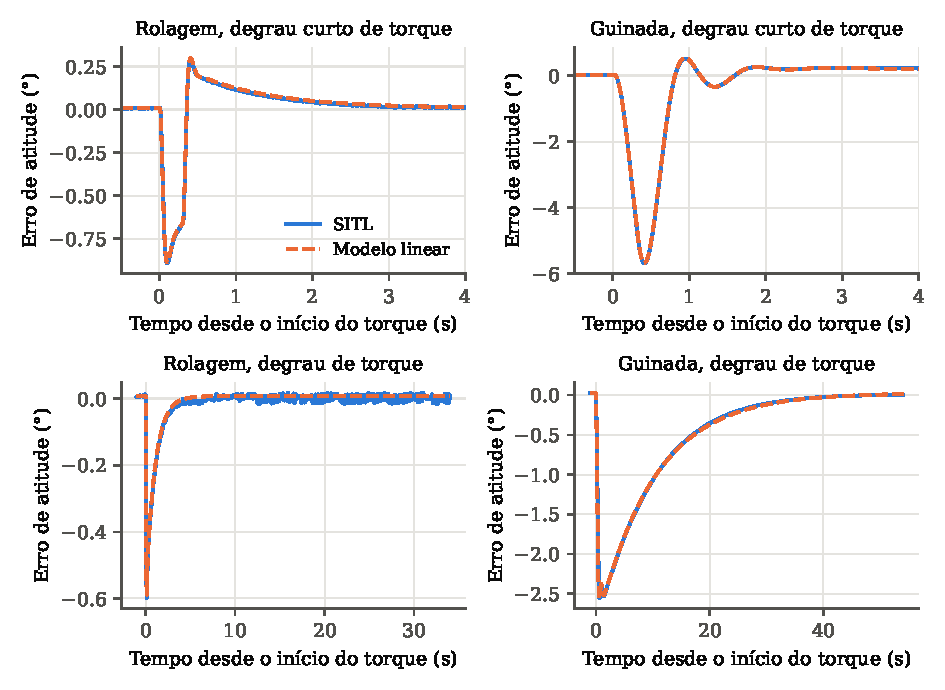
\includegraphics[width=\textwidth]{figuras/validacao_tempo}
\fonte{Elaborada pelo autor, por \codigo{modelagem/validacao.py}.}
\end{figure}

A simulação explica também a recuperação lenta da guinada. Desprezando os
filtros, a malha fechada de um eixo com o controlador de ângulo proporcional
de ganho $k$ e o PI de velocidade angular tem o polinômio característico
\begin{equation}
s^3 + (a + b\,k_P)\,s^2 + b\,(k_P\,k + k_I)\,s + b\,k_I\,k,
\label{eq:polinomio-malha}
\end{equation}
que, em guinada, tem um polo real lento próximo de $-k_I/k_P$, praticamente
independente de $a$ e de $b$. Com os ganhos gravados no voo, que a
Tabela~\ref{tab:ganhos} traz arredondados, as raízes são $-8{,}20$,
$-2{,}42$ e $\SI{-0.101}{\per\second}$, e o polo lento
tem constante de tempo de \SI{9.9}{\second}, para $k_P/k_I = \SI{10}{\second}$.
Uma exponencial com essa constante leva $\tau\ln 10 = \SI{22.8}{\second}$ para
cair a 10\,\% do pico, exatamente o tempo de recuperação do modelo e,
com 3\,\% de diferença no nativo e 3,4\,\% no \textit{backend} de exemplo, o
do SITL. A recuperação lenta não é, portanto, uma
limitação da planta, e sim consequência direta da razão $k_I = k_P/10$ que o
AutoTune impõe em guinada (Seção~\ref{sec:autotune}). Para o torque aplicado
como perturbação, o zero do PI em $-k_I/k_P$ não cancela esse polo, ao
contrário do que ocorre para um degrau de referência.

\subsection{Domínio da frequência}
\label{sec:validacao-frequencia}

Nas varreduras de torque, a resposta em frequência da perturbação para o
ângulo foi estimada pela Equação~\eqref{eq:frf}, no SITL e na simulação
alimentada pelo mesmo torque, com o mesmo método; nos dois casos, a entrada é
o torque registrado na mensagem \codigo{WND}, segurado entre as escritas do
injetor. Nos pontos em que a
coerência do SITL é de pelo menos 0,8 --- de 0,4 a \SI{9.6}{\hertz} em
rolagem e arfagem e de 0,2 a \SI{4.8}{\hertz} em guinada, praticamente toda
a faixa das varreduras ---, o modelo reproduz o ganho com diferença mediana
de no máximo \SI{0.08}{\decibel} e máxima de \SI{1.3}{\decibel}, e a fase
com diferença máxima de \ang{5.8}, em rolagem e arfagem; em guinada, as
diferenças são de \SI{0.05}{\decibel}, \SI{0.9}{\decibel} e \ang{3.2}
(Figura~\ref{fig:validacao-freq}), nos dois controladores.

\begin{figure}[htbp]
\centering
\caption{Resposta em frequência do torque para o ângulo com o PID nativo, no
SITL (pontos com coerência de pelo menos 0,8) e no modelo linear.}
\label{fig:validacao-freq}
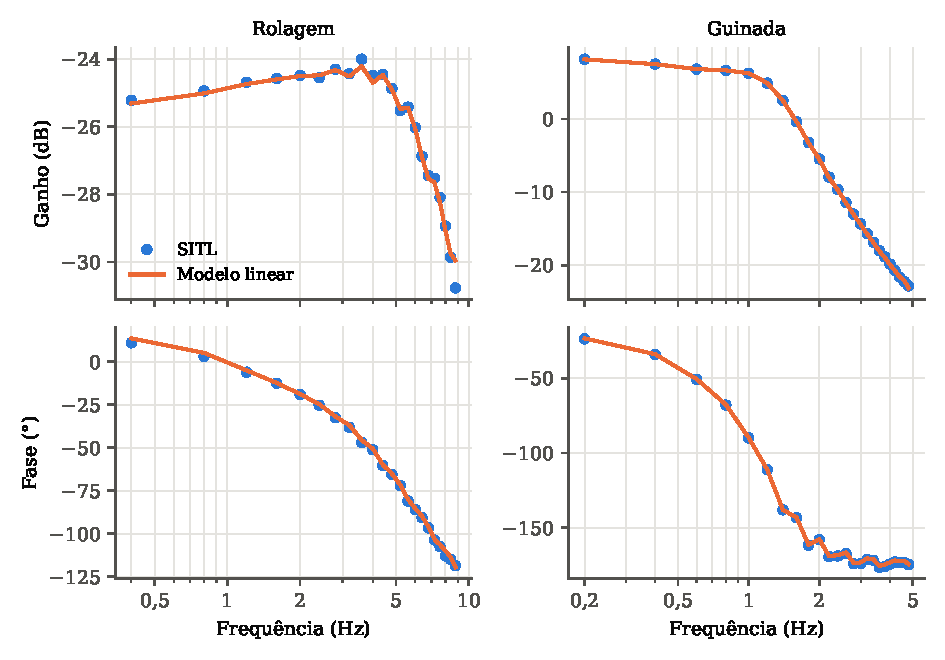
\includegraphics[width=\textwidth]{figuras/validacao_freq}
\fonte{Elaborada pelo autor, por \codigo{modelagem/validacao.py}.}
\end{figure}

As mesmas varreduras permitem identificar a planta, como prevê a
Seção~\ref{sec:identificacao}, apesar de a malha estar fechada. O torque
injetado $d$ é externo à malha e, como o ruído do giroscópio simulado é
mínimo e independente dele, não se correlaciona com nenhuma outra entrada. Dividindo a transformada de
$\dot\omega = -a\,\omega + b\,u + d$ pela de $d$, obtém-se
\begin{equation}
\mathrm{j}2\pi f\;\hat T_{d\omega}(f) - 1 = -a\,\hat T_{d\omega}(f) + b\,\hat T_{du}(f),
\label{eq:identificacao-planta}
\end{equation}
em que $\hat T_{d\omega}$ e $\hat T_{du}$ são as respostas em frequência de
$d$ para a velocidade angular e para o esforço, estimadas pelo método de
Welch contra o torque injetado. A equação é linear em $a$ e $b$, que são
obtidos por mínimos quadrados sobre os pontos de coerência de pelo menos 0,8
nas duas estimativas, separando as partes real e imaginária. A velocidade
angular registrada é a filtrada pelo passa-baixas do giroscópio, cuja
resposta em frequência é descontada de $\hat T_{d\omega}$, e os sinais são
lidos do registro a \SI{400}{\hertz}, com o torque segurado entre as escritas
do injetor, como no SITL.

Nas quatro varreduras de rolagem e arfagem, com os dois controladores, a
faixa útil vai de 0,4 a cerca de \SI{9.5}{\hertz}, com 23 ou 24 pontos. Com
$a$ e $b$ livres, $b$ sai entre 440 e \SI{446}{\radian\per\second\squared},
de 2,4\,\% a 3,6\,\% acima do previsto, mas $a$ sai negativo, entre $-1{,}5$
e $\SI{-0.06}{\per\second}$, sem significado físico. Na faixa em que a coerência
é alta, o termo $a\,\hat T_{d\omega}$ é pequeno diante de
$\mathrm{j}2\pi f\,\hat T_{d\omega}$, e os dois parâmetros se compensam: as
varreduras não identificam $a$. Fixando $a$ no valor do modelo,
$\SI{1.988}{\per\second}$, a eficácia identificada fica entre 429,5 e
\SI{432.1}{\radian\per\second\squared}, a no máximo 0,5\,\% dos
\SI{430.0}{\radian\per\second\squared} previstos.

Em guinada, a varredura começa em \SI{0.2}{\hertz}, onde $2\pi f$ é da
ordem de $a$, e os dois parâmetros se separam. Nas duas varreduras,
identificam-se $a$ entre 2,01 e $\SI{2.07}{\per\second}$, de 1\,\% a
4\,\% acima dos $\SI{1.988}{\per\second}$ previstos, e
$b_z = \SI{14.6}{\radian\per\second\squared}$, 1,4\,\% a 1,8\,\% acima
dos \SI{14.37}{\radian\per\second\squared} do modelo. As eficácias de
controle dos três eixos, parâmetros de que o projeto mais depende, estão
confirmadas dentro de 2\,\%, e o amortecimento, identificado diretamente em
guinada, onde as varreduras o alcançam, e indiretamente, pelas respostas no
tempo, em rolagem e arfagem.
